\chapter{Implementation}
\label{chp:implementation}

\section{Introduction}

A stereo vision application 

\section{Vanishing Point Detection}

\subsection{Overview}

\subsection{Line Detection}

\subsection{Line Filtering}

\subsection{Vanishing Point Detection}

\subsection{Graphical User Interface}

\begin{figure}
	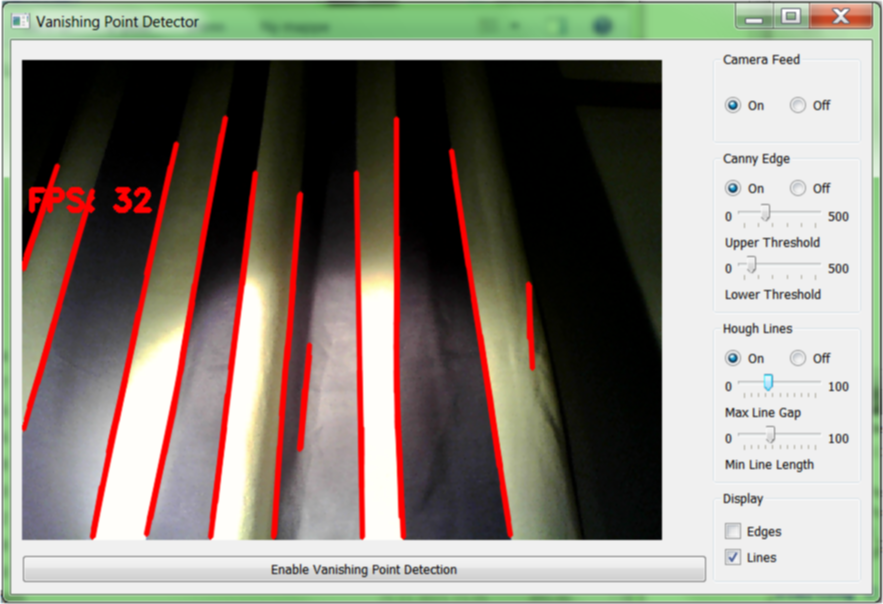
\includegraphics[scale=0.7]{VPGuiBlurred}
	\caption{Graphical user interface for the vanishing point detector.}
	\label{fig:vpGui}
\end{figure}

\subsection{Where it Fails}

\section{Depth Perception and Obstruction Detection}

\subsection{Overview}

\subsection{The camera rig}

The two IP cameras were moved together to form a stereo camera. This stereo camera was used in two positions. The first camera position is on the pan-tilt module on the robot arm, see figure \ref{fig:figure}. The second position is just over the LIDAR in front of the robot arm base, see figure \ref{fig:figure}.  The workshop at ITK made a mounting bracket, so that the cameras could be placed over the LIDAR. In stereo vision, it is essential that the positions of the cameras relative to each other is constant. One problem encountered throughout the project was that the camera assemby, when placed either at the pan-tilt module and over the LIDAR, was not rigid enough. The severity of this problem was somewhat alleviated by wrapping a strap around both the cameras. This camera rig is ad hoc, i.e. suitable for the purpose of this project, and a better solution should be used for succeeding projects.

\subsection{Graphical User Interface}

Tuning the parameters for stereo matching in OpenCV is a wearisome task, especially without a good graphical user interface. Figure \ref{fig:StereoGui} shows the user interface which was used to observe how parameter tuning alters the disparity map quality. Not all functionalities were implemented.

\begin{figure}
	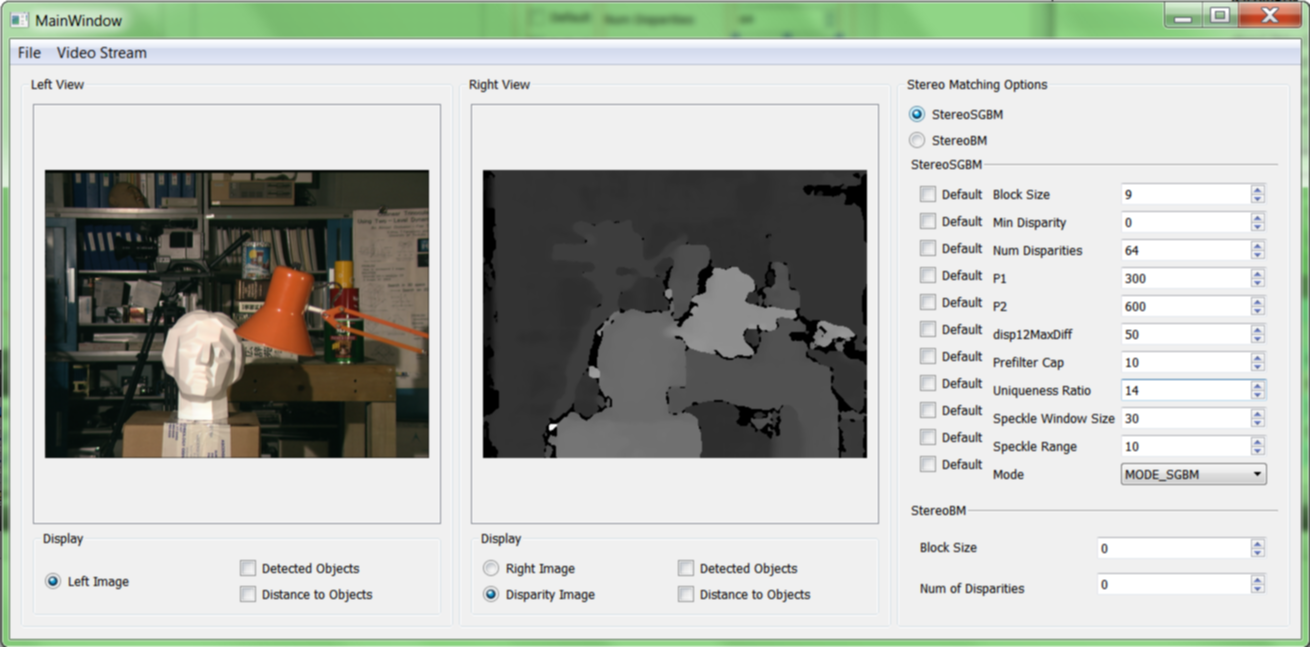
\includegraphics[scale=0.37]{StereoGui}
	\caption{Graphical user interface for stereo matching. A disparity map is computed from the Tsukuba samples by using StereoSGBM. }
	\label{fig:StereoGui}
\end{figure}

\subsection{Calibration}

As mentioned in chapter \ref{chp:theory}, all cameras will have some distortion. If the distortion is too severe, as it often will be in the context of stereo vision, the camera must be calibrated. In addition, it was assumed that the image planes were located on the same plane, and that a projection pair, for example the projections $X_L$ and $X_R$ of an object $X$, form two equal epipolar lines, $e_1$ and $e_2$, on the two image planes. In practice, these conditions are achieved through stereo calibration. The second purpose of the calibration procedure is to relate the sensor data to real world quantities, in order to measure the distance to detected objects. Code listings from Practical OpenCV by ... \cite{mal} has been used as a basis for calibration in this project. Some parts of the code is almost unchanged, while other parts of the listings are altered and expanded significantly, while the final calibration results are unchanged.


\paragraph{Single Camera Calibration}

The purpose of this calibration procedure is to counter the constant radial and tangential distortion in a pinhole camera, and to relate the image pixels to real world quantities. In this step, the cameras are calibrated separately. 



\begin{equation}
	x = x(r + t + b)
\end{equation}

\paragraph{Stereo Calibration}

\paragraph{Stereo Rectification}

%\begin{figure}
%\includegraphics[scale=•]{•}
%\end{figure}

\subsection{Stereo Matching}

\begin{figure}
\centering
 \begin{subfigure}[b]{0.45\textwidth}
        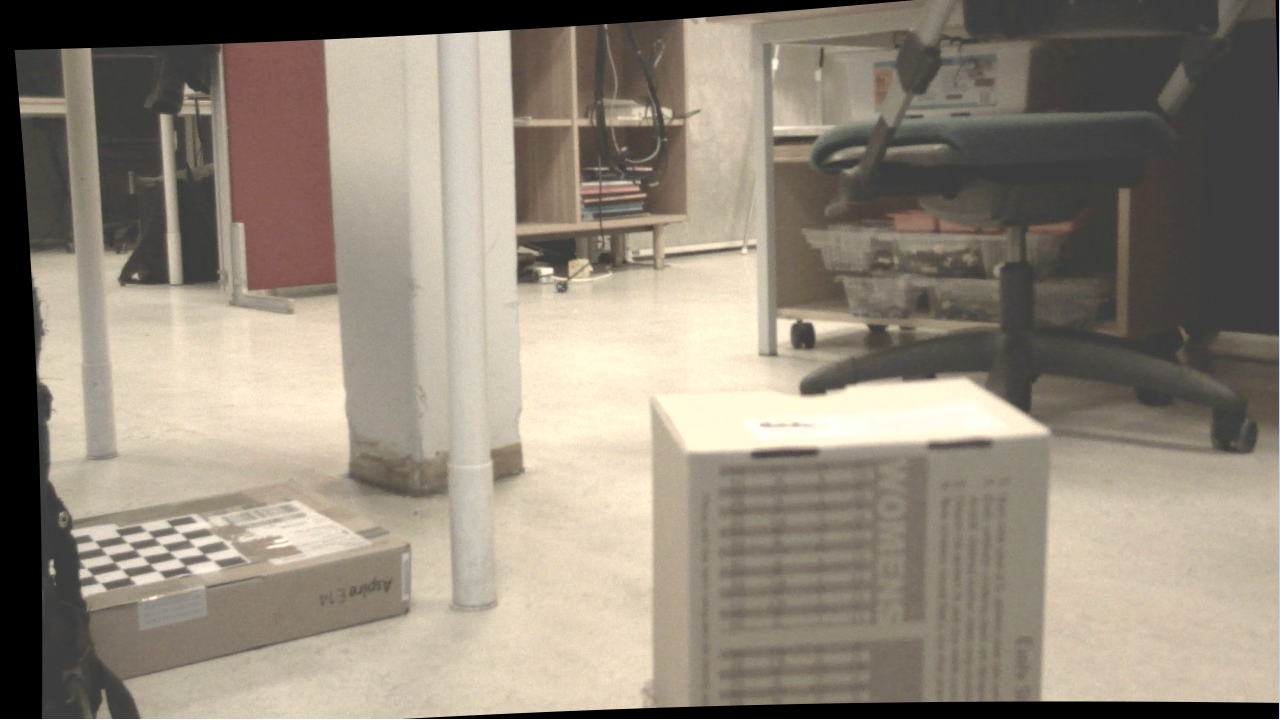
\includegraphics[width=\textwidth]{OriginalExample}
        \caption{Left camera image.}
        \label{fig:OriginalExample}
    \end{subfigure}
    \begin{subfigure}[b]{0.45\textwidth}
        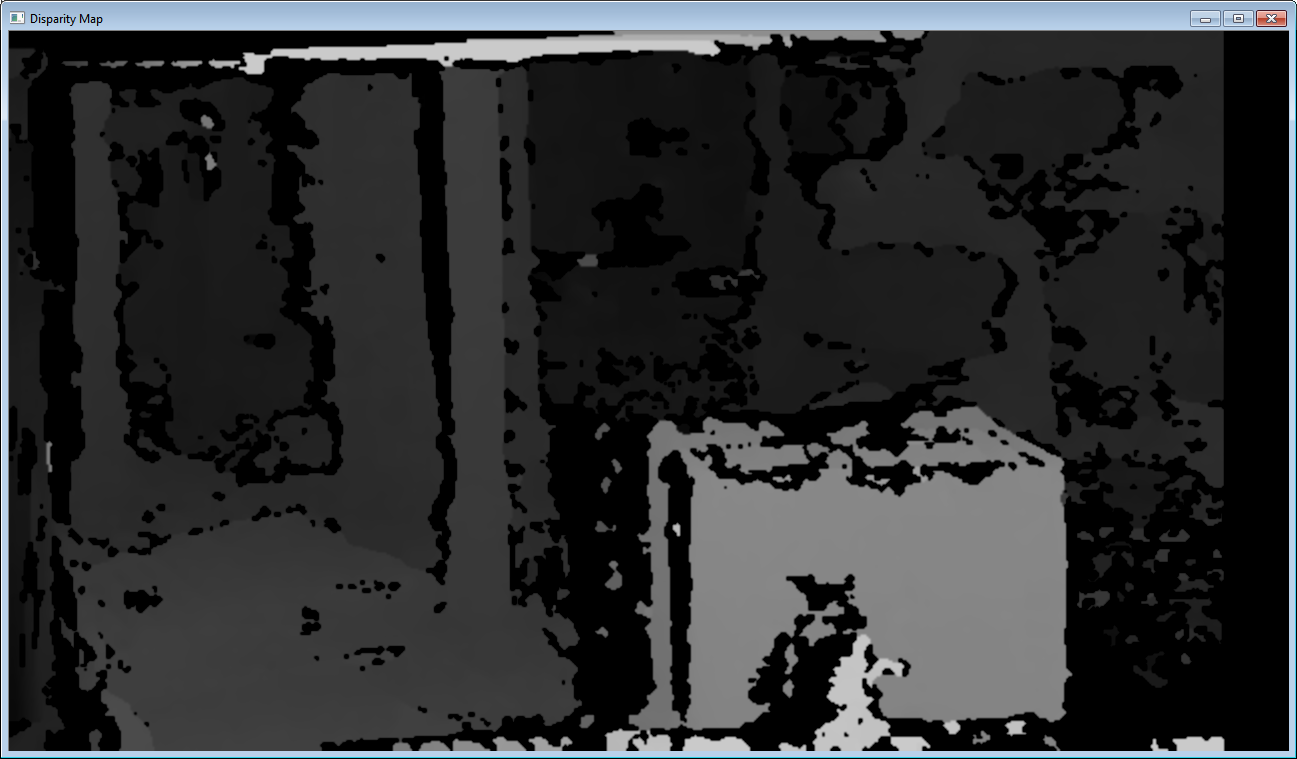
\includegraphics[width=\textwidth]{DispExample}
        \caption{Disparity map.}
        \label{fig:DispExample}
    \end{subfigure}
    \caption{\label{fig:StereoMatching}The result of StereoSGBM.}
\end{figure}

\subsection{Finding Obstructions}

\begin{wrapfigure}{r}{0.4\textwidth}
\centering
\subcaptionbox{$n = 10$ steps\label{cw_10}}{%
  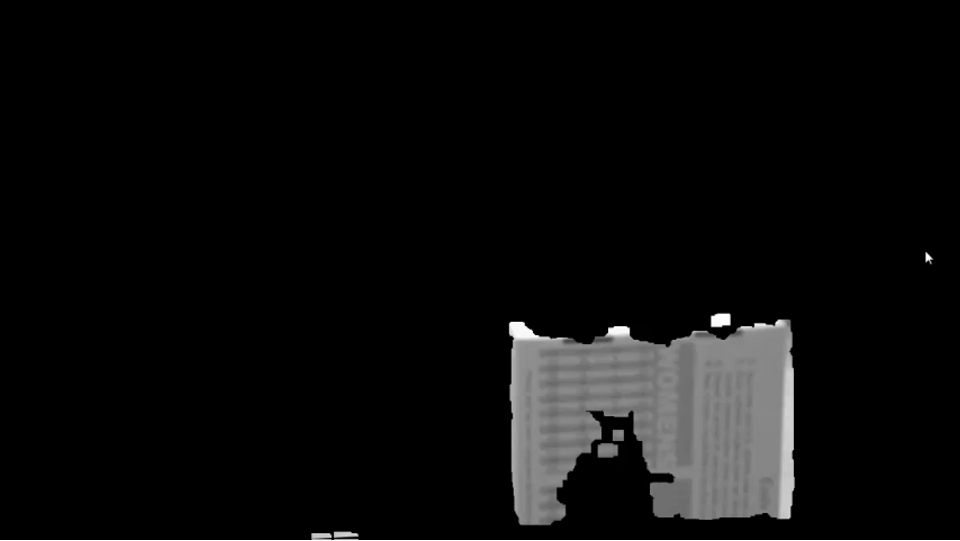
\includegraphics[width=0.4\textwidth]{DepthLayer1}%
  }\par\medskip
\subcaptionbox{$n = 25$ steps\label{cw_25}}{%
  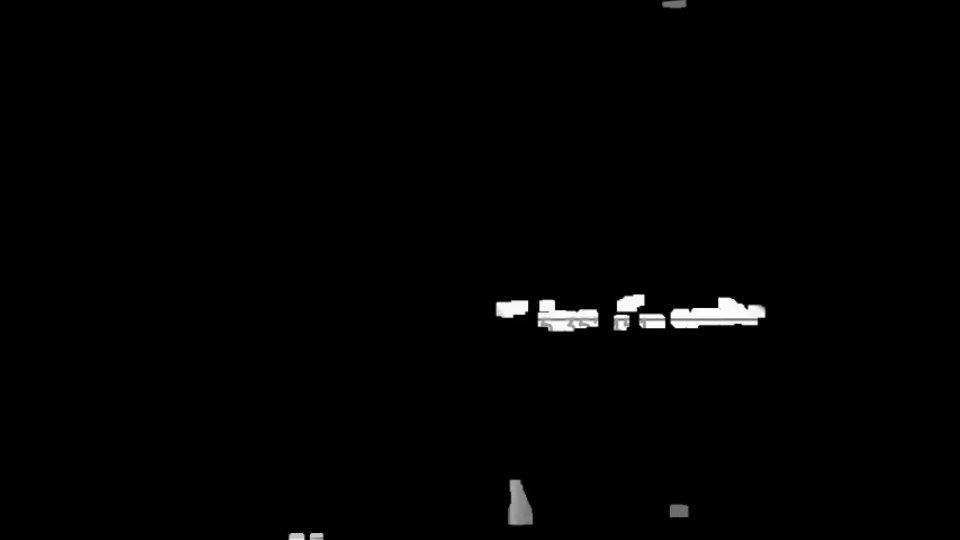
\includegraphics[width=0.4\textwidth]{DepthLayer2}%
  }\par\medskip        
\subcaptionbox{$n = 50$ steps\label{cw_50}}{%
  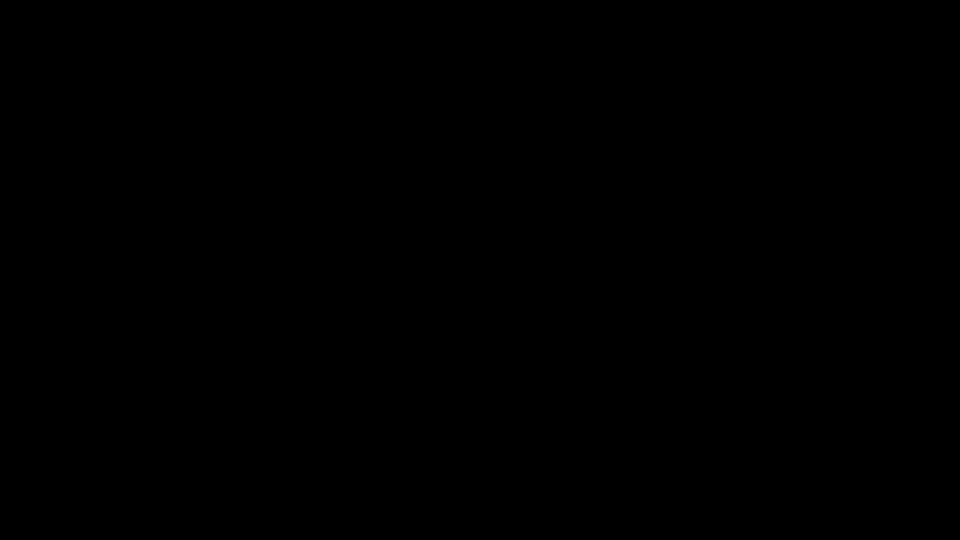
\includegraphics[width=0.4\textwidth]{DepthLayer4}%
  }
  \subcaptionbox{$n = 50$ steps\label{cw_55}}{%
  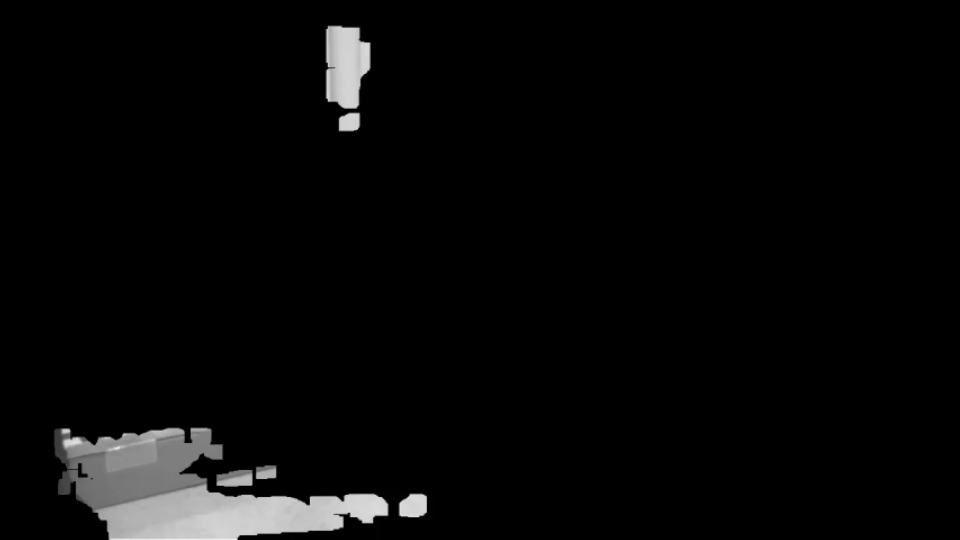
\includegraphics[width=0.4\textwidth]{DepthLayer5}%
  }
    \subcaptionbox{$n = 50$ steps\label{cw_56}}{%
  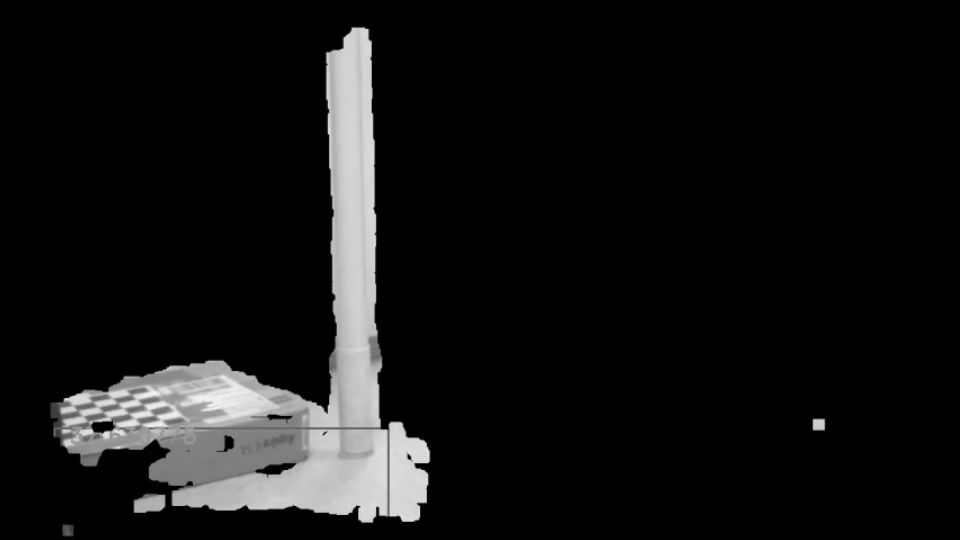
\includegraphics[width=0.4\textwidth]{DepthLayer6}%
  }
\caption{Classical Random Walk with various step sizes.}
\label{TS}
\end{wrapfigure}

\subsection{Distance Measurment}

\subsection{Problems Encountered During Implementation }